% Paste where needed in main.tex (needs \usepackage{graphicx}, already loaded).
% Use figure* for the wide ones.
\begin{figure}[t]\centering
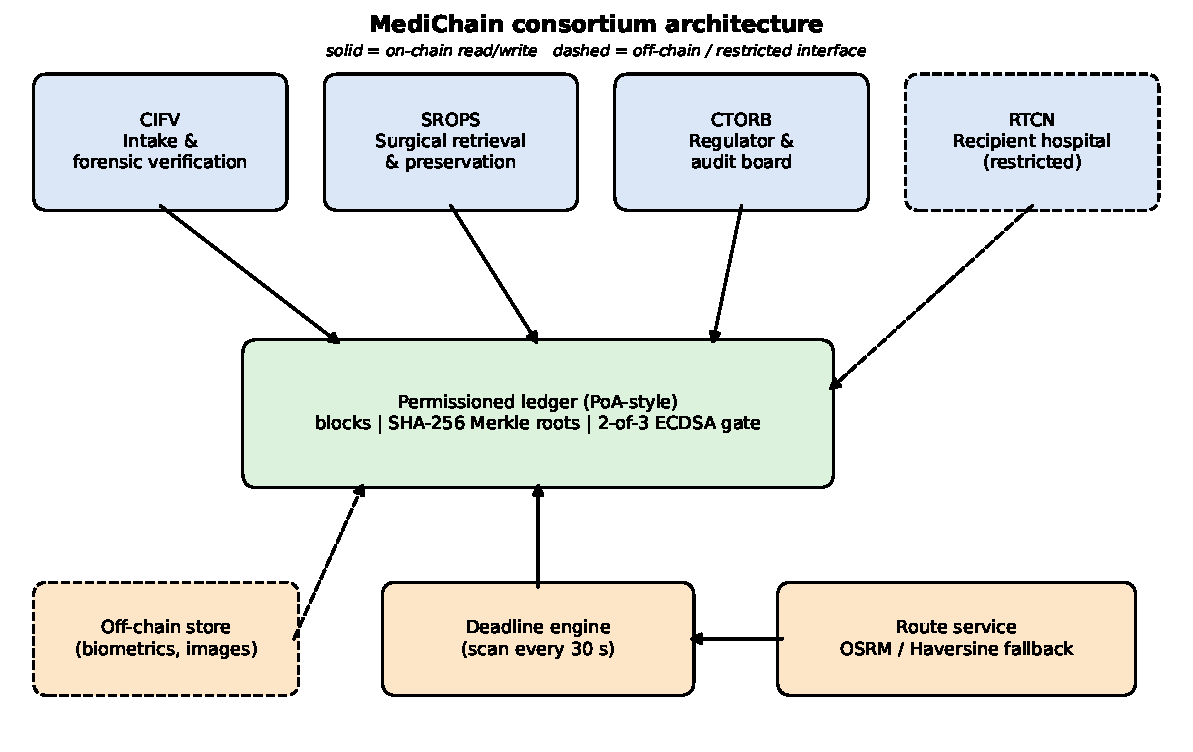
\includegraphics[width=\columnwidth]{figures/fig_architecture.pdf}
\caption{MediChain consortium architecture.}\label{fig:arch-img}\end{figure}

\begin{figure}[t]\centering
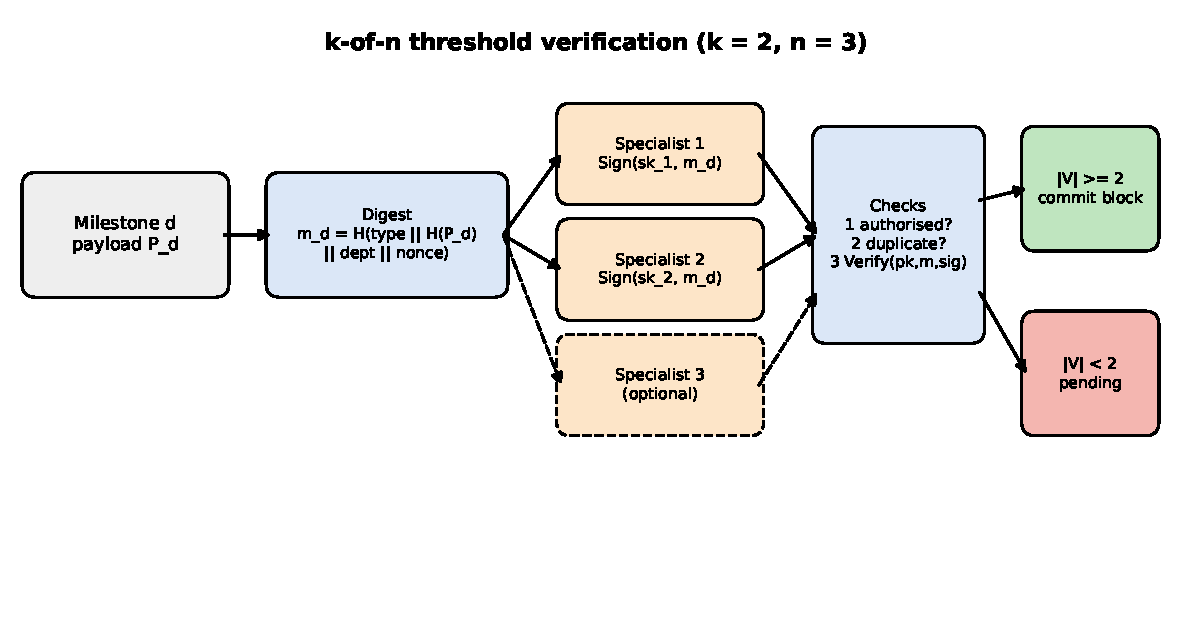
\includegraphics[width=\columnwidth]{figures/fig_threshold_flow.pdf}
\caption{2-of-3 threshold verification flow.}\label{fig:thr}\end{figure}

\begin{figure}[t]\centering
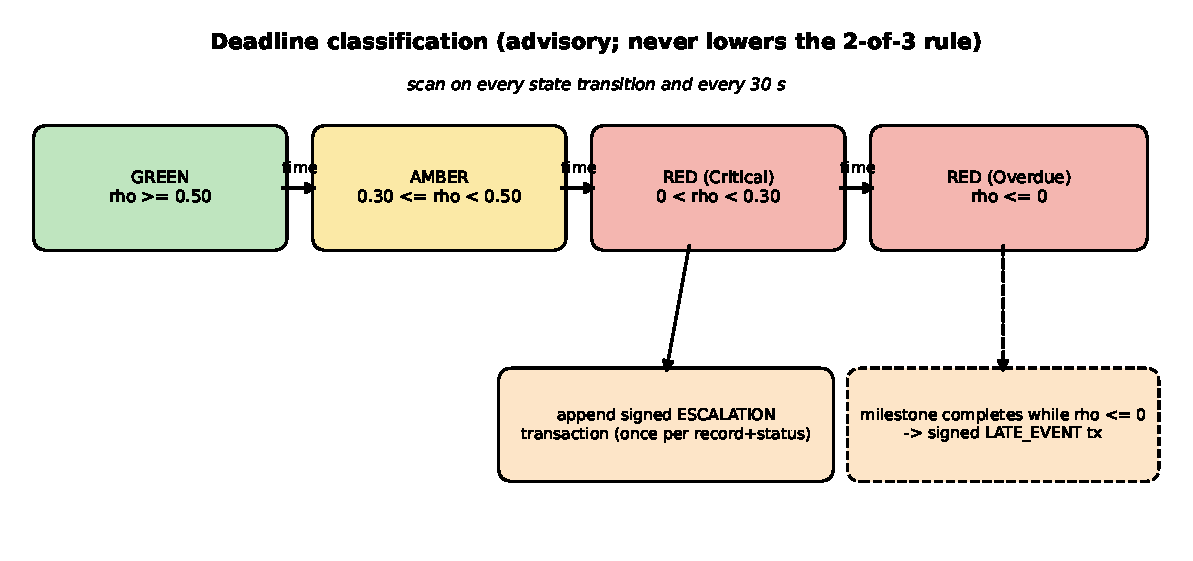
\includegraphics[width=\columnwidth]{figures/fig_deadline_states.pdf}
\caption{Deadline classification and escalation.}\label{fig:dl-img}\end{figure}

\begin{figure}[t]\centering
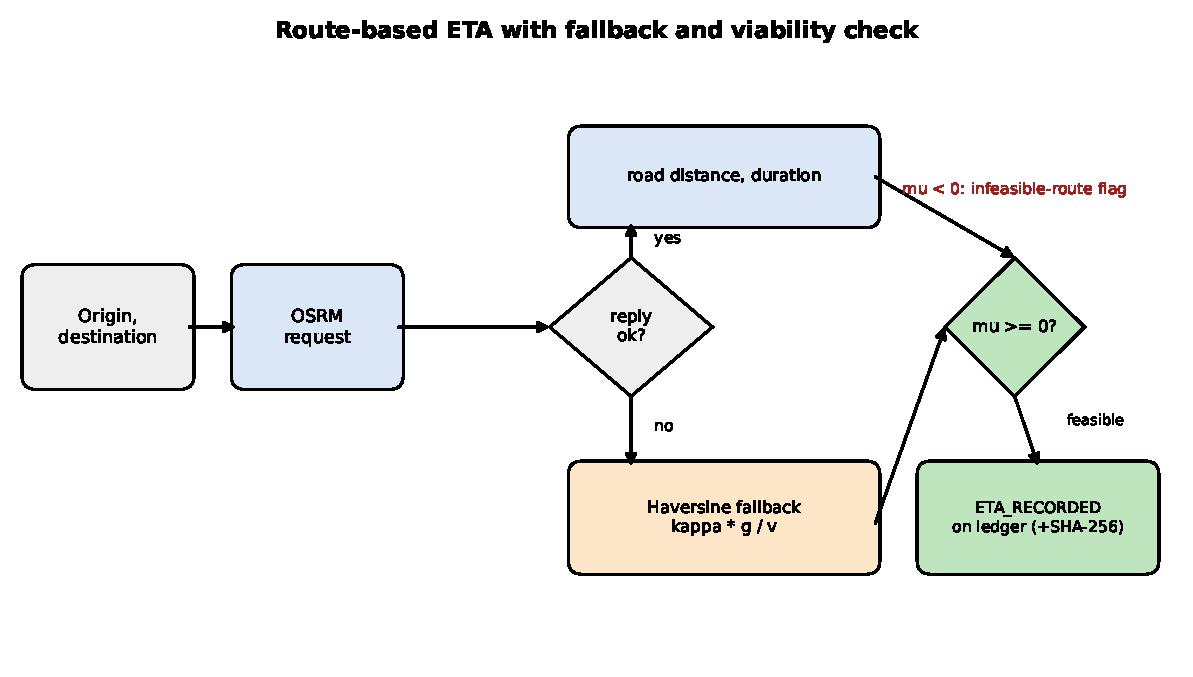
\includegraphics[width=\columnwidth]{figures/fig_eta_pipeline.pdf}
\caption{Route ETA with fallback and viability check.}\label{fig:eta-img}\end{figure}

\begin{figure}[t]\centering
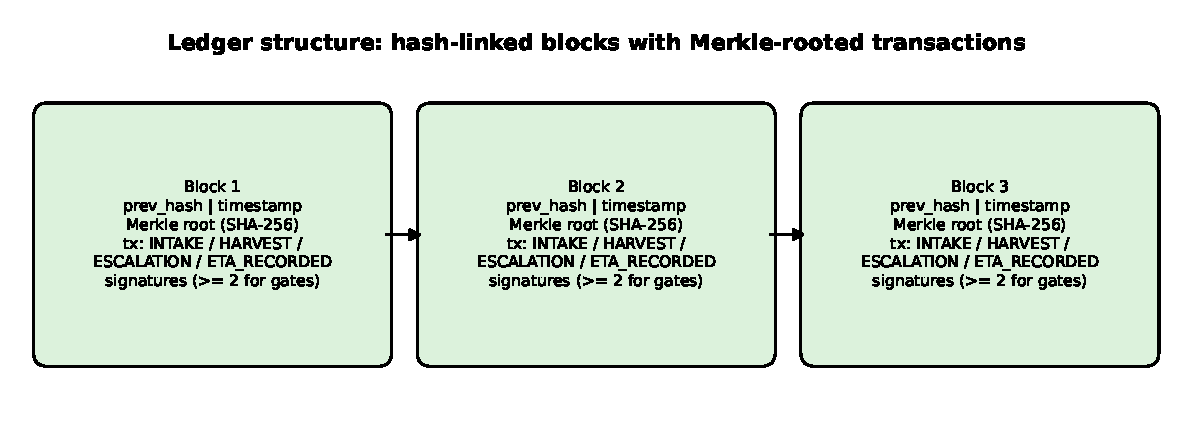
\includegraphics[width=\columnwidth]{figures/fig_ledger_blocks.pdf}
\caption{Ledger block structure.}\label{fig:blocks}\end{figure}

\begin{figure}[t]\centering
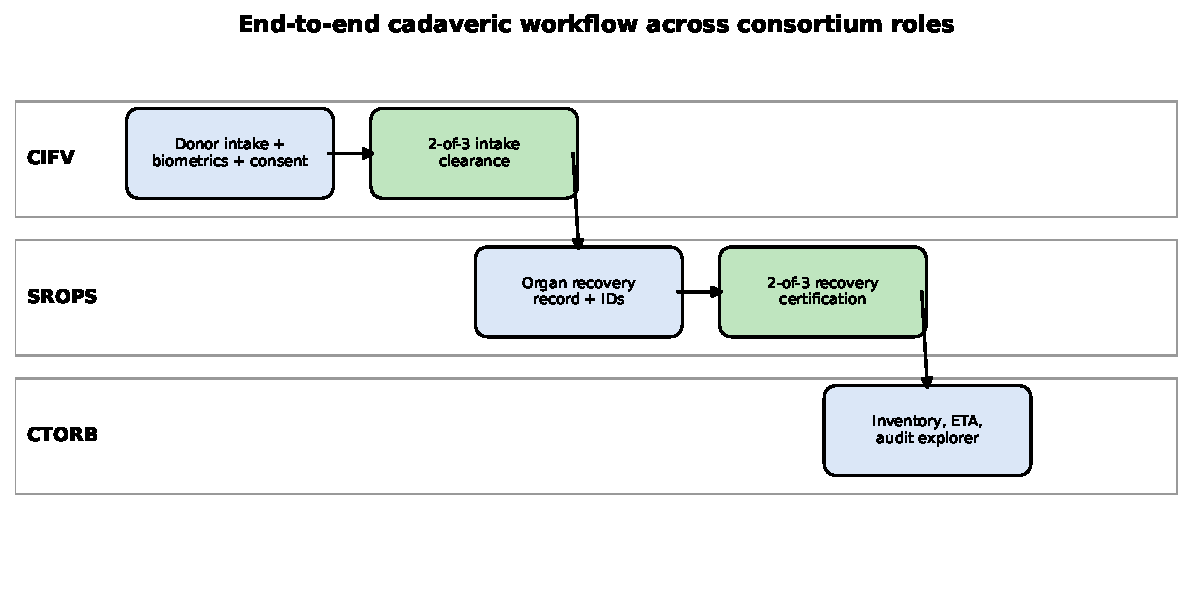
\includegraphics[width=\columnwidth]{figures/fig_workflow_swimlane.pdf}
\caption{End-to-end workflow across roles.}\label{fig:wf}\end{figure}

\begin{figure}[t]\centering
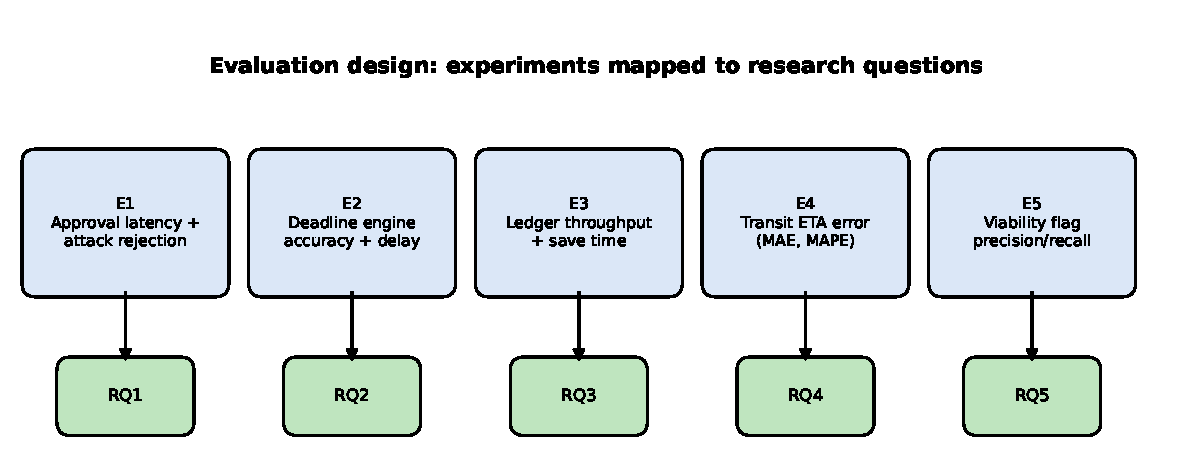
\includegraphics[width=\columnwidth]{figures/fig_evaluation_map.pdf}
\caption{Experiments mapped to research questions.}\label{fig:evalmap}\end{figure}
